\section{Analysis}\label{sec:analysis}
Firstly the data needs to be corrected because of random coincidences and misalignment of the setup. Random coincidence rate $\dot{R}$ in~\ref{math:random} is simply subtracted from the coincidence rate. In calculation of error of count rate, error of random coincidence is considered as well.

It is thought to be acceptable to just use one random coincidence rate for all angles, since it has no angular dependence. Effects of misalignment on random coincidence need to be considered. That is why the data get correction for misalignment after this step.

In figure.~\ref{fig:countRate}, one can see a clear asymmetry in count rate of the mobile detector. This can be easily explained by source not being in the center of the setup. True coincidence rate should be anti-proportional to count rates in figure.~\ref{fig:countRate}. Since measured angular correlation function is determined up to a proportional constant anyway, the normalization factor $\kappa$ is chosen to be the fraction of count rate at smallest angle and count rate at respective angle.
\begin{figure}[ht]
   \centering
   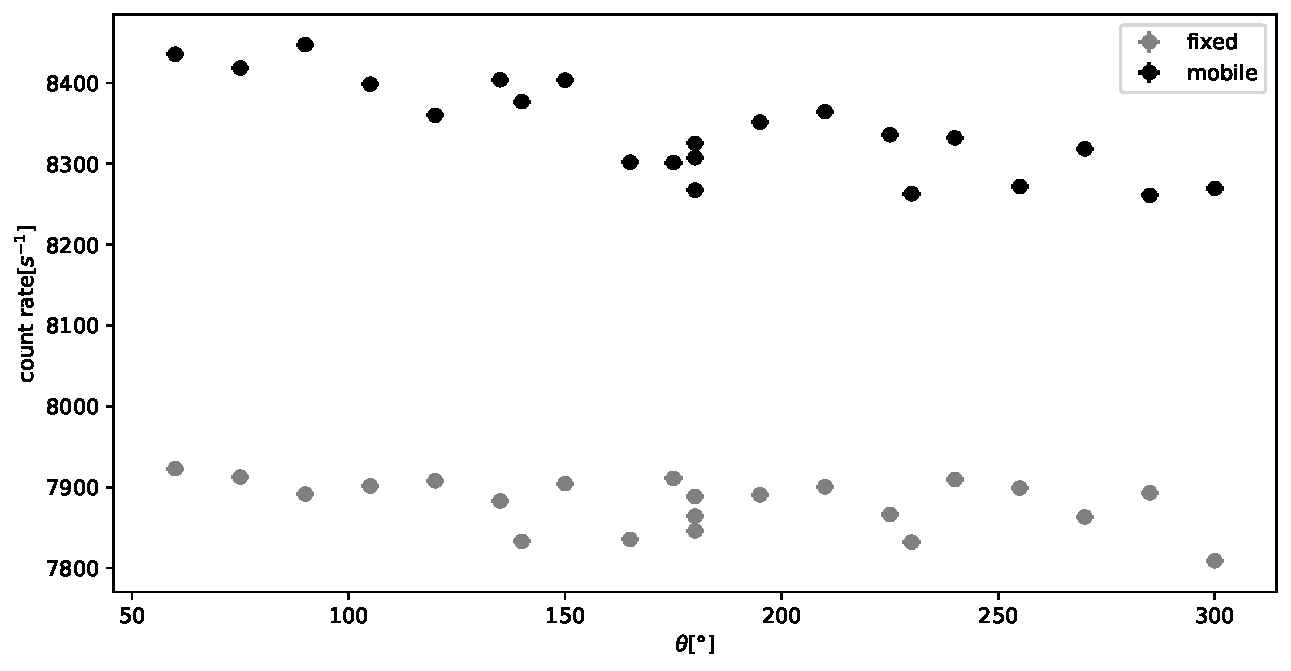
\includegraphics[width=0.8\linewidth]{./figs/countRate.pdf}
   \caption{Raw count rate}%
   \label{fig:countRate}
\end{figure}

Coincidence rates are normalized against the raw count rate with $\kappa$, in order to counter misalignment. True coincidence rate $\dot{C}_{\text{true}}$ is calculated via
\begin{equation}
   \dot{C}_\text{true} = \kappa \cdot ( \dot{C}_\text{measured} - \dot{R})
\end{equation}

During experiment, the setup and its environment might (inevitably) change, i.e.~temperature. Measurements at $180$° are repeated multiple times. Some variations have been seen. This introduces (one source of) systematic error and will be included in the further analysis.
\begin{equation}
   \Delta \dot{C}_\text{sys} = \num{0.564}
\end{equation}

Data after these corrections are plotted in figure.~\ref{fig:angCor}. Vertical error bars include statistical error and systematic error. Error of angle is estimated to be about $2$ degrees.
\begin{figure}[ht]
   \centering
   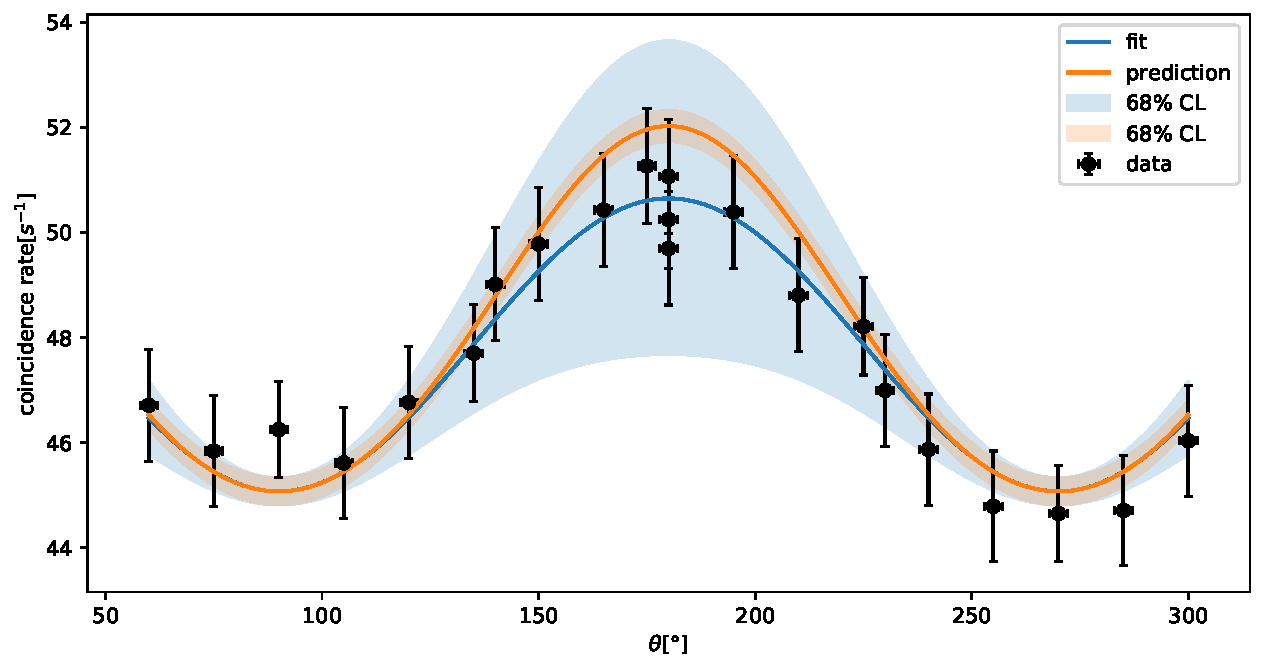
\includegraphics[width=0.8\linewidth]{./figs/angCor.pdf}
   \caption{Angular correlation with fit and prediction}%
   \label{fig:angCor}
\end{figure}

\begin{table}[ht]
   \centering
   \begin{tabular}{ccc}
      \toprule
   & fit & theory \\
      \midrule
      $A$ &\num{45.0721 +- 0.2578} &   \\
      $B$ & \num{0.1246 +- 0.0310} & \num{0.1213}\\
      $C$ &\num{-0.0008 +- 0.0289} & \num{0.0330}\\
      \bottomrule
   \end{tabular}
   \caption{Parameters of the curve shown in figure~\ref{fig:angCor} and their theoretical values after being "corrected" for finite size of detector}
   \label{tab:ABC}
\end{table}

A least squares fit of data using function in the form of \eqref{math:fTheta} is carried out. Fitted function is drawn in blue in figure~\ref{fig:angCor}. Parameters are shown in table~\ref{tab:ABC}. One should emphasize that the errors in table~\ref{tab:ABC} are only the diagonal entries of covariance matrix. There are still non-vanishing off-diagonal entries, i.e.~variables are somehow correlated. This is the reason why drawing confidence intervals in figure ~\ref{fig:angCor} is not meaningful. Covariance matrix of these fitting parameters is
\begin{equation}
   \Sigma_{ABC} = \begin{pmatrix} \num{0.06648601} & \num{-0.00610261} & \num{0.00462504} \\
   \num{-0.00610261} & \num{0.00096016} & \num{-0.00086438} \\
\num{0.00462504} & \num{-0.00086438} & \num{0.00083277}\end{pmatrix}
\label{math:Sigma}
\end{equation}

Based on this value of $A$, we can plot the predicted function equation~\eqref{math:pred}. Because of finite size of detector, prediction curve needs to be "corrected" by factor $Q_k$ to correspond measured correlation curve. It is more convenient to apply this correction to fit curve than data points. Values of $Q_k$ are taken from~\cite{siegbahn} with distance to source $h=\SI{5}{\cm}$. Energy of $\gamma$-radiation in experiment is between \SI{1}{\mega\eV} and \SI{1.5}{\mega\eV} and only photopeaks are relevant. For convenience, mean values of $Q_k$ of these two energies are used in calculation
\begin{equation*}
   Q_2 = \num{0.934},\; Q_4 = \num{0.792}
\end{equation*}
Theoretical prediction with $Q$ correction of fit parameters are also added in table ~\ref{tab:ABC}.

It seems that prediction and measurement have at least OK agreement, only some deviation around \SI{180}{\degree} is present. But a closer look is necessary, since the fit parameters are correlated. For simplicity, we say that $A$ has no correlation to other parameters and only its best-fit value is used. This will underestimate "distance" between theory and measurement. Taking only $B$ and $C$ components of equation~\eqref{math:Sigma}, one can draw confidence intervals on parameter plane.
\begin{figure}[ht]
   \centering
   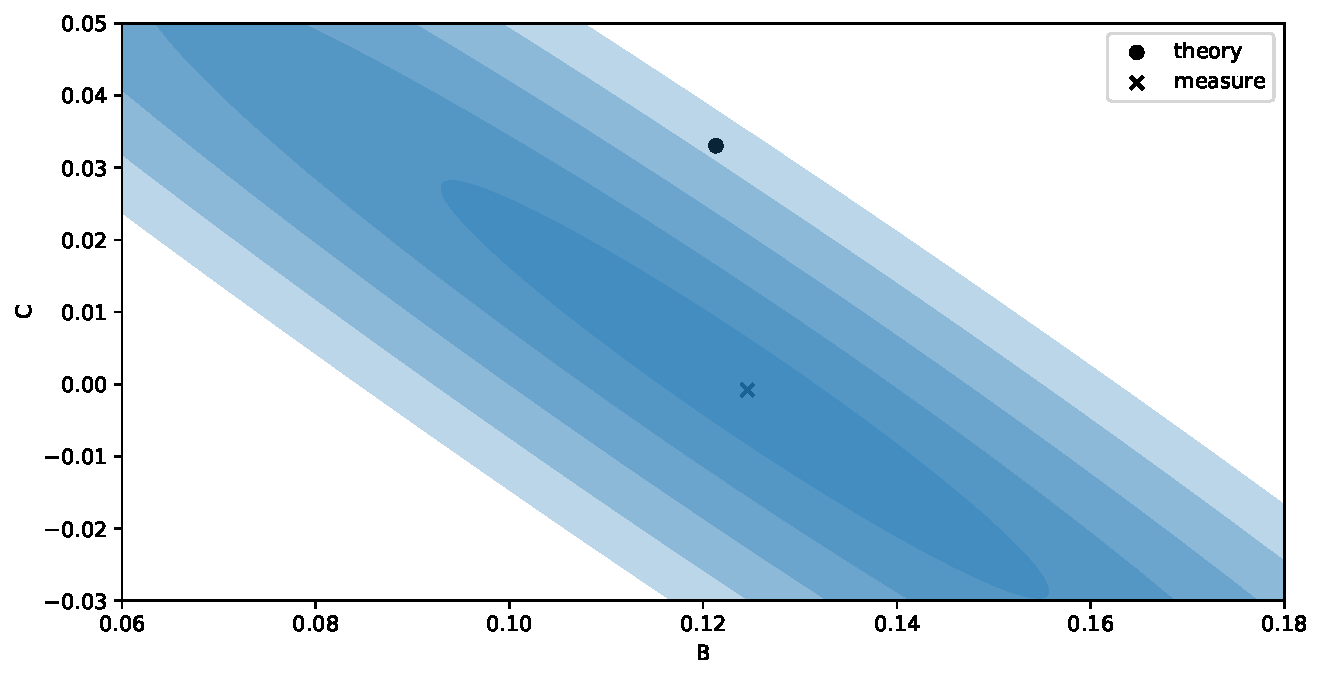
\includegraphics[width=0.8\linewidth]{./figs/BCpara.pdf}
   \caption{Regions on the plane $(B,C)$ measured by experiment. Best-fit and theoretical prediction are included. The contours corresponds to $1\sigma$, $2\sigma$, $3\sigma$, $4\sigma$, $5\sigma$ confidence intervals. }%
   \label{fig:BCpara}
\end{figure}
In figure~\ref{fig:BCpara}, one can see prediction value lie roughly $4\sigma$ away from best-fit value, even though table~\ref{tab:ABC} gives us roughly $1\sigma$ accuracy.

Just as a consistency check and to better understand origin of deviation, $B$ and $C$ can be converted into $\alpha$, $\beta$ like before.
\begin{equation}
   \begin{pmatrix} \alpha \\ \beta \end{pmatrix} = 
   \begin{pmatrix} 1 & 1 \\ 1 & -1\end{pmatrix} 
   \begin{pmatrix} B \\ C \end{pmatrix}
\end{equation}
\begin{table}[ht]
   \centering
   \begin{tabular}{ccc}
      \toprule
   & fit & theory \\
   \midrule
      \alpha & \num{0.1238} & \num{0.1544} \\
      \beta & \num{0.1254} & \num{0.0883} \\
      \bottomrule
   \end{tabular}
   \caption{Prediction and measurement of $\alpha, \beta$. Here theoretical value has been corrected by $Q$-factor.}
   \label{tab:alphabeta}
\end{table}

Results are in table~\ref{tab:alphabeta}. Their covariance matrix is
\begin{equation*}
   \Sigma_{\alpha\beta} = \begin{pmatrix} \num{6.41664749e-05} & \num{1.27395676e-04} \\ \num{1.27395676e-04} & \num{3.52169920e-03} \end{pmatrix}
\end{equation*}
Thus deviations are present at all angles, not e.g.~only around \SI{180}{\degree} when only $\alpha$ is off.

There is quite obvious asymmetry (with respect to \SI{180}{\degree}) present in the angular correlation. Ideally, this should not be in data, or at least after being corrected by considering misalignment. To better see the difference, data points are plotted in figure.~\ref{fig:angAsymm}. From this, we can see that the asymmetry can be well explained by the errors.
\begin{figure}[ht]
   \centering
   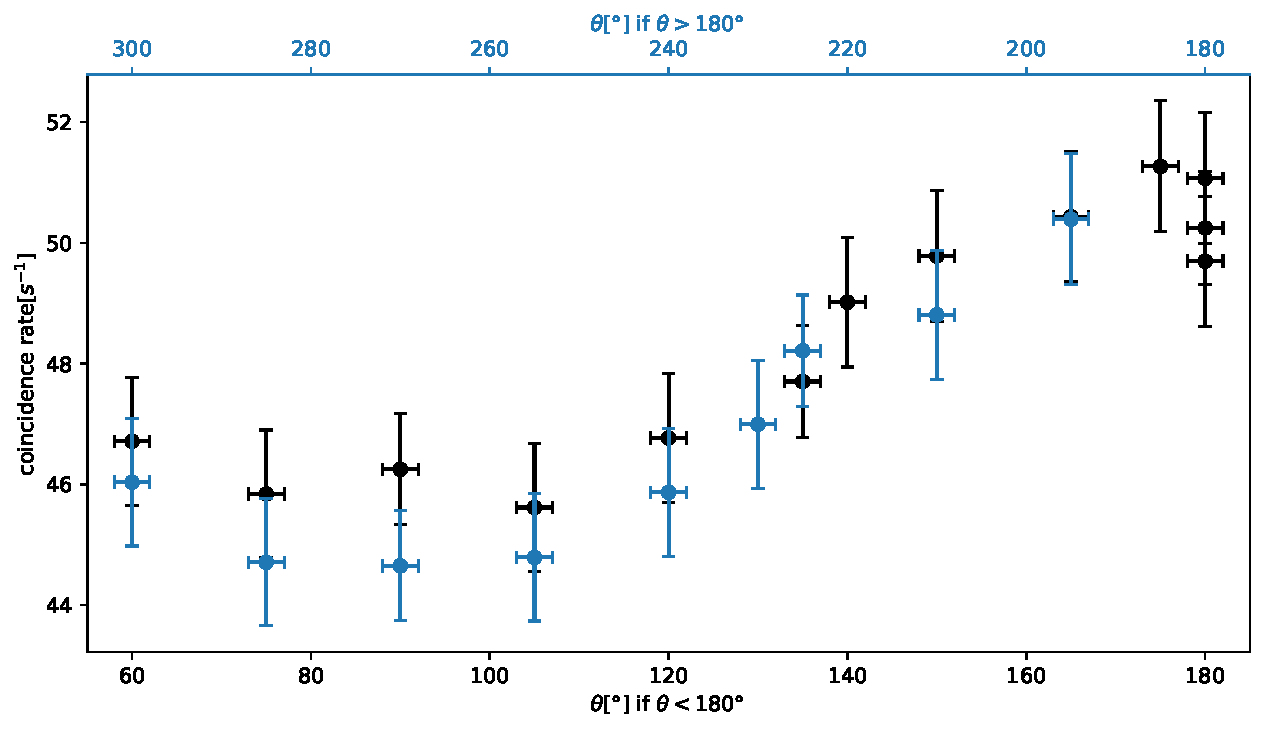
\includegraphics[width=0.8\linewidth]{./figs/angAsymm.pdf}
   \caption{Angular correlation to see asymmetry. Color of data points correspond to the color of axis to use.}%
   \label{fig:angAsymm}
\end{figure}

They need to be converted to $A_{kk}$ coefficients and then corrected for finite size of detectors. As written in equation~\eqref{math:pred}, both $A_{22}$ and $A_{44}$ decides the values of $B$ and $C$ (need to scale it, so that the constant term is unity!). Thus it involves finding the inverse of the matrix. The errors here are given without correlation considered, i.e.~these are only diagonal entries of covariance matrix.
\begin{table}[htpb]
   \centering
   \label{tab:Akk}
 \begin{tabular}{ccc}
   \toprule
   &  fit with correction &  theory \\
   \midrule
   $A_{22}$ & \num{0.0849 +- 0.0057} & 0.1020 \\
   $A_{44}$  & \num{-0.0002 +- 0.0063}& 0.0091 \\
   \bottomrule
\end{tabular}
\caption{Measured coefficients after corrected for finite size of detectors and theoretical values}
\end{table}

Fitting of angular correlation could also help us to exclude other cascades. From previous found values of $B$ and $C$, one can conclude that $020$, $121$, $220$, and $320$ cascades are pretty much $100 \%$ excluded using coefficients provided by~\cite{deutsch}. Alternatively, fit function can also only contain $\cos^2\theta$ term. This fit curve visually doesn't differ from the previous curve visually, as expected since $C$ from previous fit is almost vanishing. New fit parameters are
\begin{table}[ht]
   \centering
   \begin{tabular}{cc}
      \toprule
   & fit  \\
      \midrule
      $A$ &\num{45.0765 +- 0.1969} \\
      $B$ & \num{0.1237 +- 0.0077} \\
      \bottomrule
   \end{tabular}
   \caption{Parameters using alternative fit function. Errors are just the diagonal entries of covariance matrix.}
   \label{tab:ABC}
\end{table}
Comparing this $B$ to values give in~\cite{deutsch}, the closest (positive) value is of $210$ and $220$ cascades with $B=3/7\approx\num{0.43}$. Although $Q$ correction is not included, we know for sure $Q \sim 1$, and measured value is no way near \num{0.43} (more than dozens of $\sigma$s away). Some negative values are numerically closer to measured value. But from the plot, coefficient $B$ is obviously positive. We can say for sure, measured angular correlation does not correspond to any other cascades listed in~\cite{deutsch}.
